\section{\textsc{Porting Process}}
\label{sec:porting_process}

\subsection{Target version}
\label{sec:target_version}

The original version of the sandbox is based on Android 2.3.4, one of
the earliest versions of the Google OS. Nowadays Gingerbread is
largely outdated and accounts for only 0.8\% in the Android platforms
distribution \cite{ref16}. The main drawback of having an outdated version at
the dynamic analysis core is that the API level, used by the sandbox,
does not supporting most of the applications. Applications, in fact,
contain in their manifest file an integer value called \textit{minSdkVersion}
which expresses the minimum API level required to run the application
\cite{ref17}. Developers, as a consequence, are not interested in creating
apps compatible with an Android version with 0.8\% of
market share. The \textsc{TraceDroid} compatibility rate, as a consequence,
decreases drastically.

We, hence, decided to port the system to an higher Android version to
increase the compatibility rate with applications to be dynamically
analyzed. We have chosen Android KitKat as the target version (Android
4.4, API level 19). The main reason for this choice is that version
4.4 is the last one still using the Dalvik Virtual Machine as default
runtime environment. In KitKat the VM is now implemented in
C{}\verb!++! instead of C but the file structure and the functions
provided are similar, making the porting process
smoother. Furthermore, the market share of this platform is
18.1\%, corresponding to the third most used Android version. Developers,
being aware of the data, are interested in supporting this major
version and hence most applications will have at least version 19 or
lower as \textit{minSdkVersion} in their manifest file. As a
consequence porting \textsc{TraceDroid} to Android 4.4, despite not
being the latest Android version, will increase the compatibility rate
significantly.

\subsection{Porting tools}
\label{sec:porting_tools}

The first step into porting \textsc{TraceDroid} was to setup a build
environment to download the Android source tree from Google git
repository and to compile it to obtain a default system image. The
source code can be compiled only under Linux or Mac OS. On top of this
Google suggests to use Ubuntu 64-bit as the default Linux distribution
to build Android \cite{ref18}. We chose to use a docker container as a build
environment for Android 4.4 to avoid dependencies issues on the client
Linux machine we were working from. We selected Ubuntu 12.04 64-bit
image from the official Ubuntu docker repository because of its
compatibility with Google mobile OS older versions. We then
downloaded the Android source code \cite{ref19} and successfully compiled it after
solving the dependencies issues causing compilation errors. The
technical details regarding the dependencies installed in the docker
container for compiling both Gingerbread and KitKat can be found in
the Github repository of the project \cite{ref15}.

We needed to install also the Android SDK tools \cite{ref21} to be able to emulate
an Android system image. We performed this by installing Android
studio and the required dependencies in our client Linux machine, in
the specific \textit{debian 3.16.0-4-amd64} \cite{ref20}. The SDK tools allowed
us to create an Android Virtual Device (AVD) to hold the system image
with its properties and then emulate it \cite{ref15}. This was fundamental to
access our custom \textsc{TraceDroid} system image and interact with
it via the \texttt{adb} (Android Debug Bridge) command line interface
\cite{ref22}.

\subsection{Porting workflow}
\label{sec:porting_workflow}

\textsc{TraceDroid} \cite{ref1} performs the tracing by modifying the behavior of the
virtual machine containing the application that we want to analyze
dynamically. The changes, hence, involve the files under the
\texttt{dalvik/vm/} folder in the Android source code. The first stage in the
porting process was to understand the difference between the original
\textsc{TraceDroid} \texttt{dalvik/vm/} files and the original ones of Android 2.3.4,
the Android version on which it is based. We used the \texttt{diff} command
recursively between the two folders to keep track of all the
differences at the source code level.

The second stage was to port the changes step by step to the
\texttt{dalvik/vm/} source files of Android 4.4. The modifications were ported
together with the addition of debugging messages to the Android logs
via the \texttt{ALOGD} macro. After performing every step in the porting
process we pushed the implemented files to the docker image
responsible of building the sources. We compiled the \texttt{dalvik/vm/} module
with the \texttt{mm} utility and then linked it to the other modules with the
\texttt{make} command executed at the root of the Android source tree. After the compilation was
terminated we pulled the generated system image from the container and
we emulated it. We started some activities to trigger \textsc{TraceDroid} and
analyzed the logs after it was terminated. In the case there were no
compile or runtime errors and the system was behaving as expected, the
next modifications could be applied. In case of errors, we rolled back the
applied changes and performed bug tracking and bug fixing. The diagram
showing the workflow of the porting process can be seen in figure~\ref{fig:porting_workflow}.

\begin{figure}[!h]
    \centering
    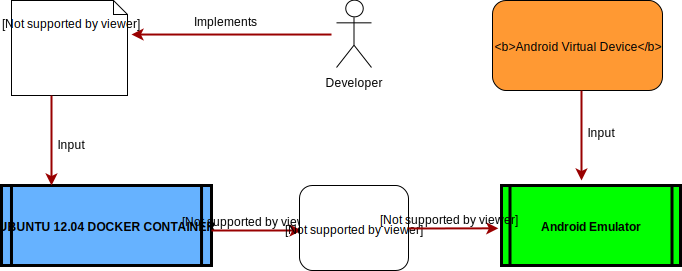
\includegraphics[width=1\textwidth]{./img/porting/flowDiagram.pdf}
    \caption{Workflow Diagram}
    \label{fig:porting_workflow}
\end{figure}

\subsection{Porting steps}
\label{sec:porting_step}

We explain in this section the incremental steps taken to perform the
porting process. We describe them in a chronological order as follows:

\paragraph{Enabling tracing for a specified app} ~\\
We added to the file \texttt{Globals.h} the variables to deal with the
common interface to specify which app to track. The variables hold the
uid file containing the application uid to be dynamically
analyzed. We modified the \texttt{Init.cpp} file to implement the
functionality of reading the \texttt{/sdcard/uid} file and starting the
tracing in case an app with that unique identifier is launched.

\paragraph{Entering method, exiting method and exception throwing capturing} ~\\
\texttt{dvmMethodTraceAdd()} is the method in \texttt{Profile.cpp}
responsible for intercepting the calls to enter or exit a method and
also the thrown exceptions. Every time this method is called, the
action integer-type parameter holds one of the three values, defined
by three different macros, specifying what kind of call is caught. In
this step we added to \texttt{Profile.cpp} the code to analyze this
value and, depending on that to call, a method to handle the case. The
three methods to work with the three different possibilities were also
added, namely \texttt{handle\_method}, \texttt{handle\_return} and
\texttt{handle\_throws}.

\paragraph{Getting method indentation and timestamps} ~\\
In this phase we added the integer-type depth variable to the
\texttt{Thread.h} header to hold the indentation level. This value is
increased before calling \texttt{handle\_method} and decreased before
calling either \texttt{handle\_return} or \texttt{handle\_throws}. The
\texttt{getWhitespace()} method was then ported and the calls to this
method added in the three handle ones in order to print correctly the
indentation level and the timestamps.

\paragraph{Getting method modifiers, return type and class descriptor} ~\\
The functions to get the called method modifiers calculated by
\texttt{getModifiers()}, the return type and the class descriptor,
both computed by \texttt{convertDescriptor()}, were ported at this
stage. The calls to these function were added to
\texttt{handle\_method}.

\paragraph{Retrieving parameters types and values} ~\\
First the \texttt{parameterToString()} method was ported to get a
string representation of a parameter containing both its type and its
value. Second the \texttt{getParameters()} method, that iteratively
computes the string representations of all the parameters, was implemented. This
is accomplished by calling the previously described method for each
parameter. The array containing the parameters' string representation
is then returned. Last the \texttt{getParameterString()} function was
implemented. It gives a string representation of the array computed by
\texttt{getParameters()}. The calls to these computational procedures
were then added to \texttt{handle\_method} with an additional check to
call them only in case there are parameters to be computed.

\paragraph{Retrieving exceptions and return value} ~\\
To compute the string representation of a thrown exception or a
returning value we first needed to modify the header declaration
(\texttt{Profile.h}) regarding
\texttt{dvmMethodTraceAdd()}. Furthermore, we also redefined the two
macros responsible of calling this method in case of exception or
returning method, respectively \texttt{TRACE\_METHOD\_UNROLL} and
\texttt{TRACE\_METHOD\_EXIT}. The modification was implemented by
adding an extra value to hold either the thrown exception or the
returning value. The new parameter was also added to
\texttt{handle\_return} and \texttt{handle\_throws}. The returning
value or the exception risen was added as parameter to 
the macros called when unrolling or exiting a method. We added, as a last step, in
\texttt{handle\_return} and \texttt{handle\_throws} respectively
\texttt{parameterToString()} and \texttt{convertDescriptor()}
functions to get a string representation of the returning value and
the exception.

\paragraph{Printing the traces to \texttt{/sdcard/}} ~\\
First the file pointer to the output file and the lock to perform the
writing were added to \texttt{Thread.h}. The \texttt{prep\_log()}
function was implemented in \texttt{Profile.cpp} in order to create
the traces in files that follows the format
\texttt{dump.ProcessID.ThreadID}. The \texttt{ALOGD\_TRACE} macro was
declared in the \texttt{Profile.h} header to actually print the
retrieved values to the appropriate dump file. The last step was to
add this macro to the three handle methods functions to print the
values calculated by the previously ported functions.
